\section{Web application}
\label{sec-webapplication}

The developed web application consists of three main part: back-end (server side), front-end (client side) and tool 
for Geant4 tests configuration. The data flow between application components is shown on the Fig.~\ref{fig:dataflow}.

\begin{figure}[h]
    \centering
    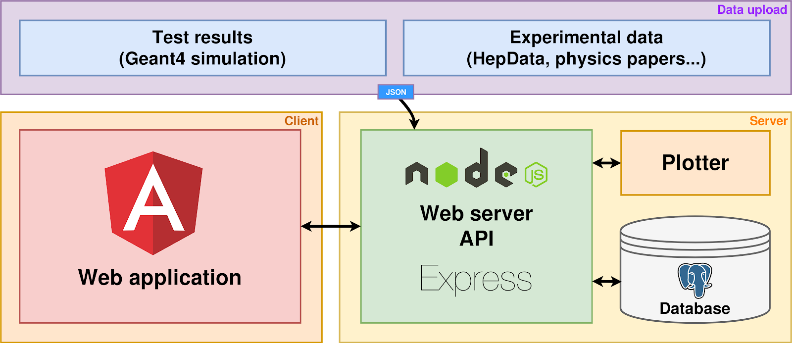
\includegraphics[width=0.8\textwidth,clip]{schema.png}
    \caption{Data flow between application components.}
    \label{fig:dataflow}
\end{figure}

The server is the core of the Geant4 validation system. It provides a web API allowing clients to access the database, responding to the clients requests and generates high quality plots "on the fly" using ROOT~\cite{ROOT} whenever they are requested. PostgreSQL is used as database management system and provided by CERN Database-On-Demand service.

The server is written in JavaScript and run under Node.js engine. Node.js has an event-driven architecture capable of asynchronous I/O. These design choices aim to optimize throughput and scalability in web applications with many input/output operations, as well as for real-time Web applications.

Database schema is designed in a way to allow storing scatter plots and histograms with unlimited number of parameters. Currently the application's database contains 86213 tests histograms/charts and 1414 experimental data ones.

To produce high quality plots ROOT based C++ utility is developed. It uses data in the application's JSON format (see Appendix~\ref{adx:JSON-format}) which has been introduced as main data interface between all parts of the application. The plotter utility is not deeply integrated in the server infrastructure and can be used as a standalone application if one wish to plot data locally. It supports scatter plots and 1D histograms with ability to plot on one canvas histograms with different binning and/or ratio plots. Plot axes ranges and scales are selected automatically, with ability to override them if necessary. User-defined styles (in ROOT terms) are also supported.

The second part of the validation application is front-end which is an AngularJS single page application (SPA).
AngularJS is chosen because it allows to fastly build efficient web applications with highly reusable components.
The website contains 4 pages:

\begin{itemize}
    \item User layouts
    \item Statistical comparison
    \item Experimental data
    \item Page to search values in the application's database
\end{itemize}

"User layouts" page (see Fig.~\ref{fig:layouts}) is designed for visual comparison of set of plots. It is possible to compare different versions between them and against experimental data. Also users can define their own templates and use them on the page. 
If two or more Geant4 versions are selected, one can also enable plotting the ratio.

\begin{figure}[h]
    \centering
    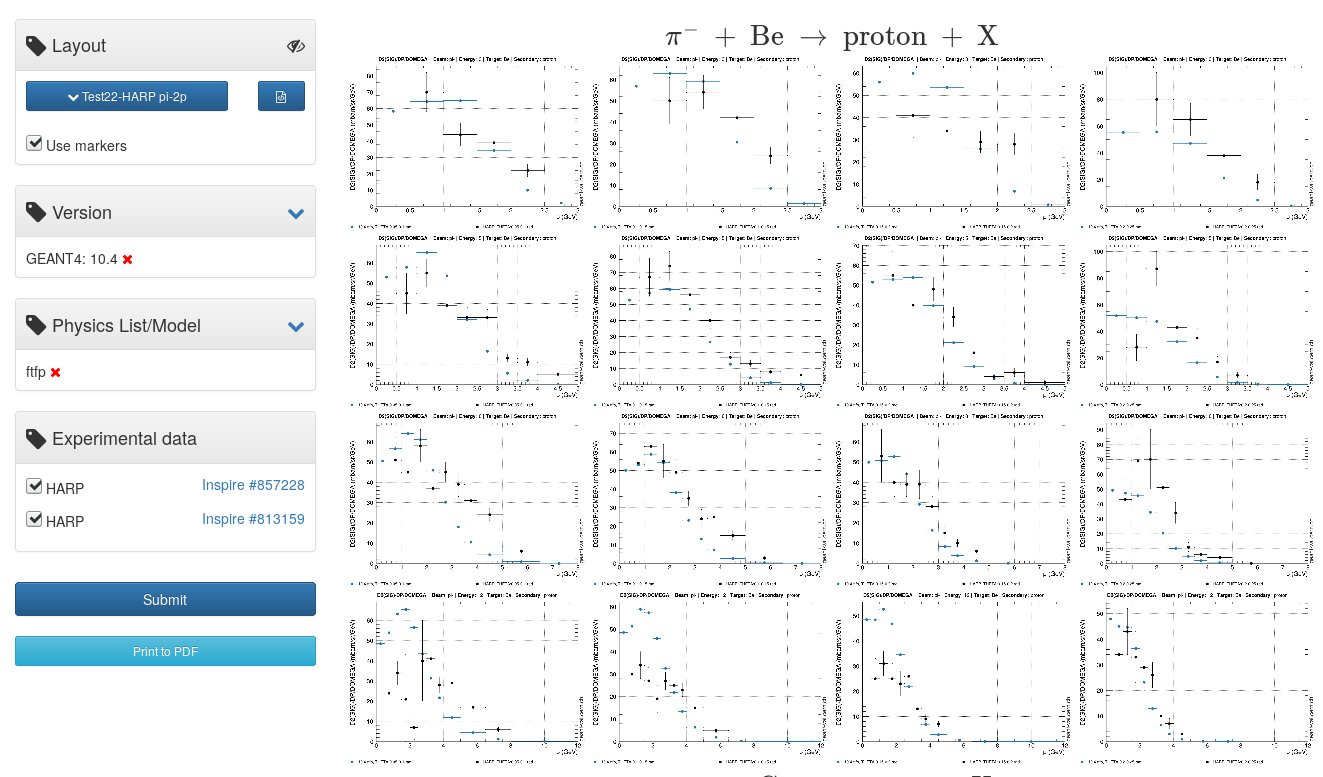
\includegraphics[width=0.8\textwidth,clip]{layouts.png}
    \caption{User layouts.}
    \label{fig:layouts}
\end{figure}

"Statistical comparison" page (see Fig.~\ref{fig:statcomparison}) allows performing statistical validation of Geant4 and experiments for given test. It displays pairs of plots for different versions with the same parameter values. For these pairs results of $\chi^2$ and Kolmogorov-Smirnov (KS) tests are displayed ($\chi^2/n.d.f.$, $\chi^2$ probability, KS and KS $\mathrm{Max(D)}$). All computations are performed on the client side in separate browser's processes using JavaScript WebWorkers API.
For this purpose $\chi^2$ and Kolmogorov-Smirnov tests have been reimplemented in JavaScript and validated against ROOT framework.

\begin{figure}[h]
    \centering
    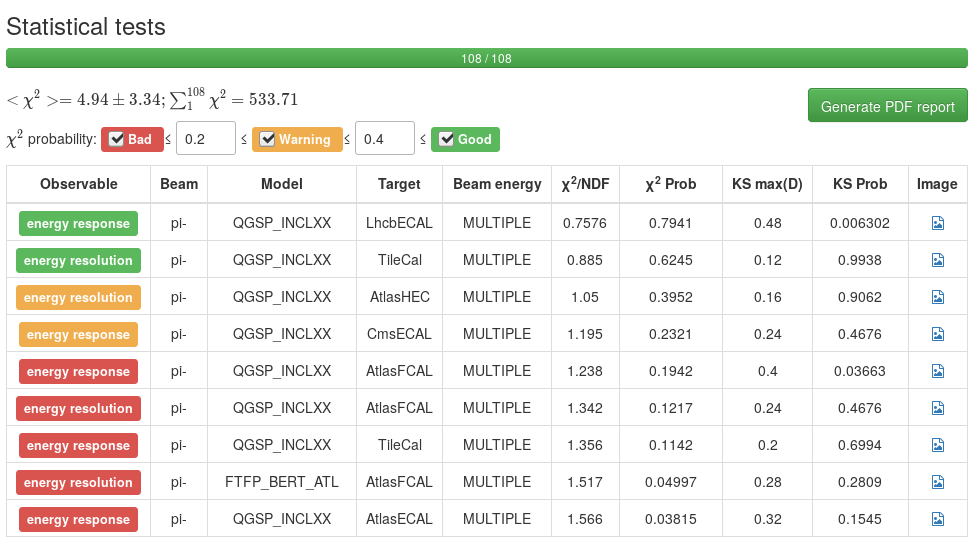
\includegraphics[width=0.8\textwidth,clip]{statcomparison.png}
    \caption{Statistical comparison.}
    \label{fig:statcomparison}
\end{figure}

On the "experimental data" page (see Fig.~\ref{fig:exppage}) a summary table of available experimental data is displayed. In the application experimental data is not linked with particular test and can be used by any tests if target, particles, observable and parameters match with simulation data.
"Lookup table" page contains all predefined values, such as project names, versions, observables, particles, etc.

\begin{figure}[h]
    \centering
    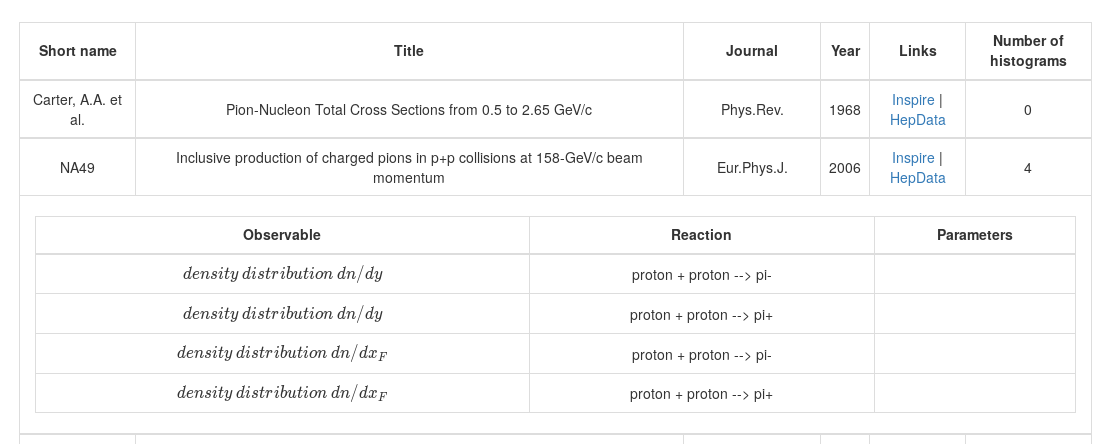
\includegraphics[width=0.8\textwidth,clip]{expdata.png}
    \caption{Available experimental data.}
    \label{fig:exppage}
\end{figure}

Each plot in the application can be viewed in static and interactive mode using JSROOT~\cite{JSROOT}, which allows changing axes ranges, scales and styles of the data "on the fly" in the same way as it can be done in ROOT. It is possible to export the plots in PNG, ROOT or EPS format to use them in articles or reports. For testing purposes the website also provides JSON and Gnuplot output.

In order to restrict access to Geant4 testing releases, the application uses user authorization based on CERN Single-Sign-On service.

%Don't forget to give each section, subsection, subsubsection, and
%paragraph a unique label (see Sect.~\ref{sec-1}).

%For one-column wide figures use syntax of figure~\ref{fig-1}
%\begin{figure}[h]
% Use the relevant command for your figure-insertion program
% to insert the figure file.
%\centering
%\includegraphics[width=1cm,clip]{tiger}
%\caption{Please write your figure caption here}
%\label{fig-1}       % Give a unique label
%\end{figure}

%For two-column wide figures use syntax of figure~\ref{fig-2}
%\begin{figure*}
%\centering
% Use the relevant command for your figure-insertion program
% to insert the figure file. See example above.
% If not, use
%\vspace*{5cm}       % Give the correct figure height in cm
%\caption{Please write your figure caption here}
%\label{fig-2}       % Give a unique label
%\end{figure*}

%For figure with sidecaption legend use syntax of figure
%\begin{figure}
% Use the relevant command for your figure-insertion program
% to insert the figure file.
%\centering
%\sidecaption
%\includegraphics[width=5cm,clip]{tiger}
%\caption{Please write your figure caption here}
%\label{fig-3}       % Give a unique label
%\end{figure}

%For tables use syntax in table~\ref{tab-1}.
%\begin{table}
%\centering
%\caption{Please write your table caption here}
%\label{tab-1}       % Give a unique label
% For LaTeX tables you can use
%\begin{tabular}{lll}
%\hline
%first & second & third  \\\hline
%number & number & number \\
%number & number & number \\\hline
%\end{tabular}
% Or use
%\vspace*{5cm}  % with the correct table height
%\end{table}